\begin{apendicesenv}

\partapendices \chapter{Backlog do Produto Inicial} \label{apendice_backlog_inicial}

\begin{figure}[H]
    \centering
    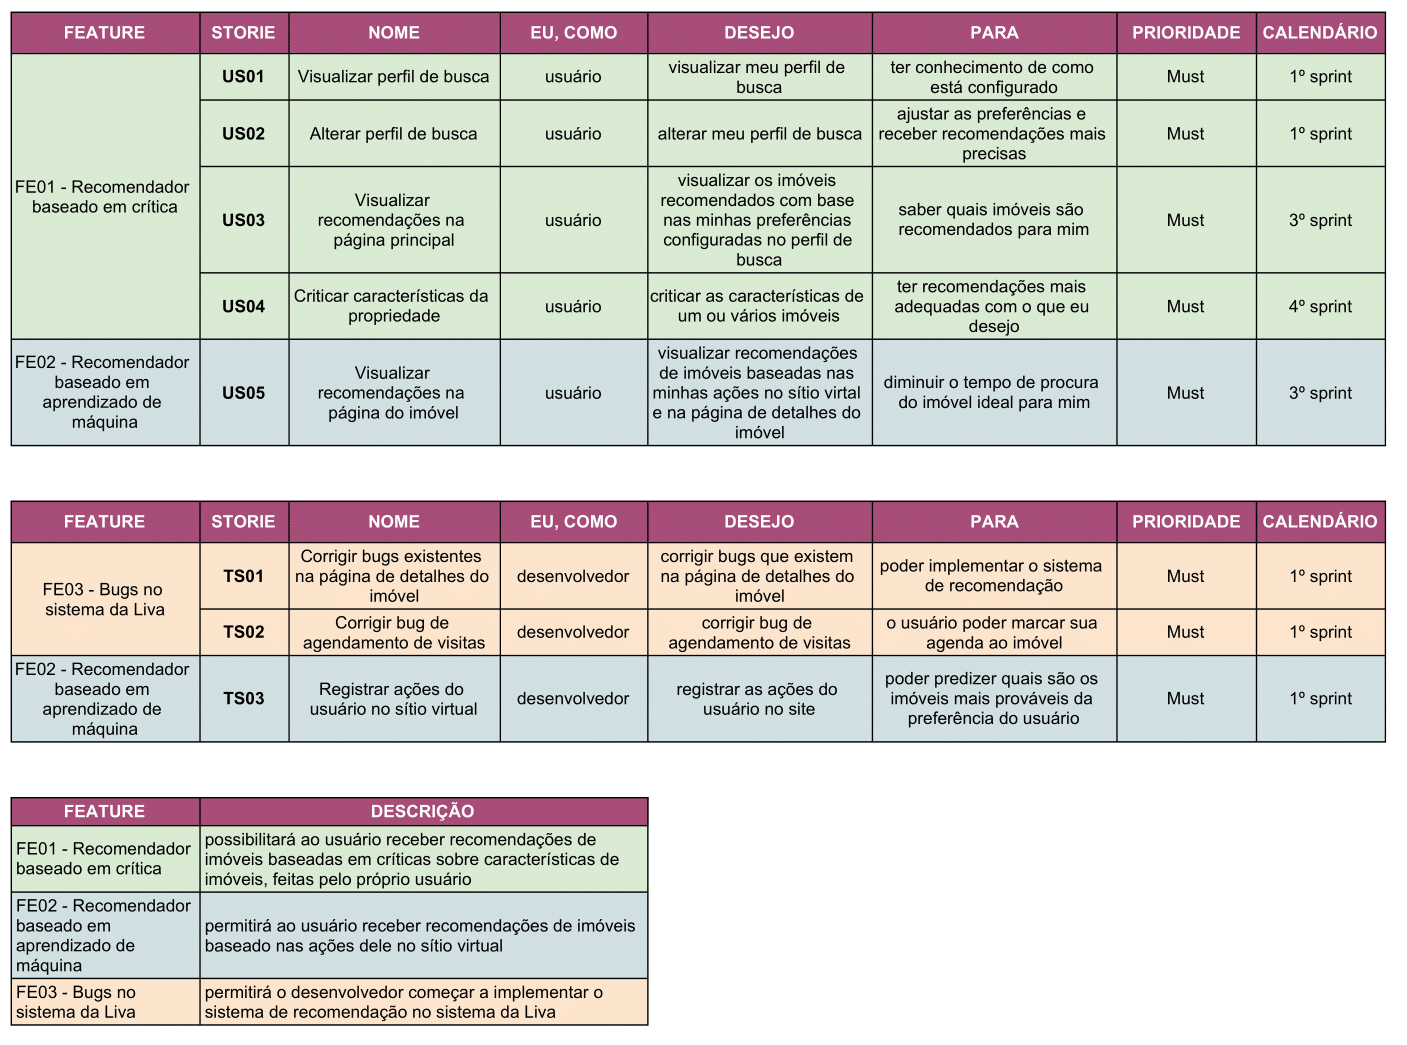
\includegraphics[scale=0.32]{figuras/desenvolvimento/backlog-v1.png}
    \caption[Backlog do produto inicial]{Backlog do produto inicial.}
    \label{fig:apendice_backlog_inicial}
\end{figure}

\chapter{Backlog do Produto final} \label{apendice_backlog}

\begin{figure}[H]
    \centering
    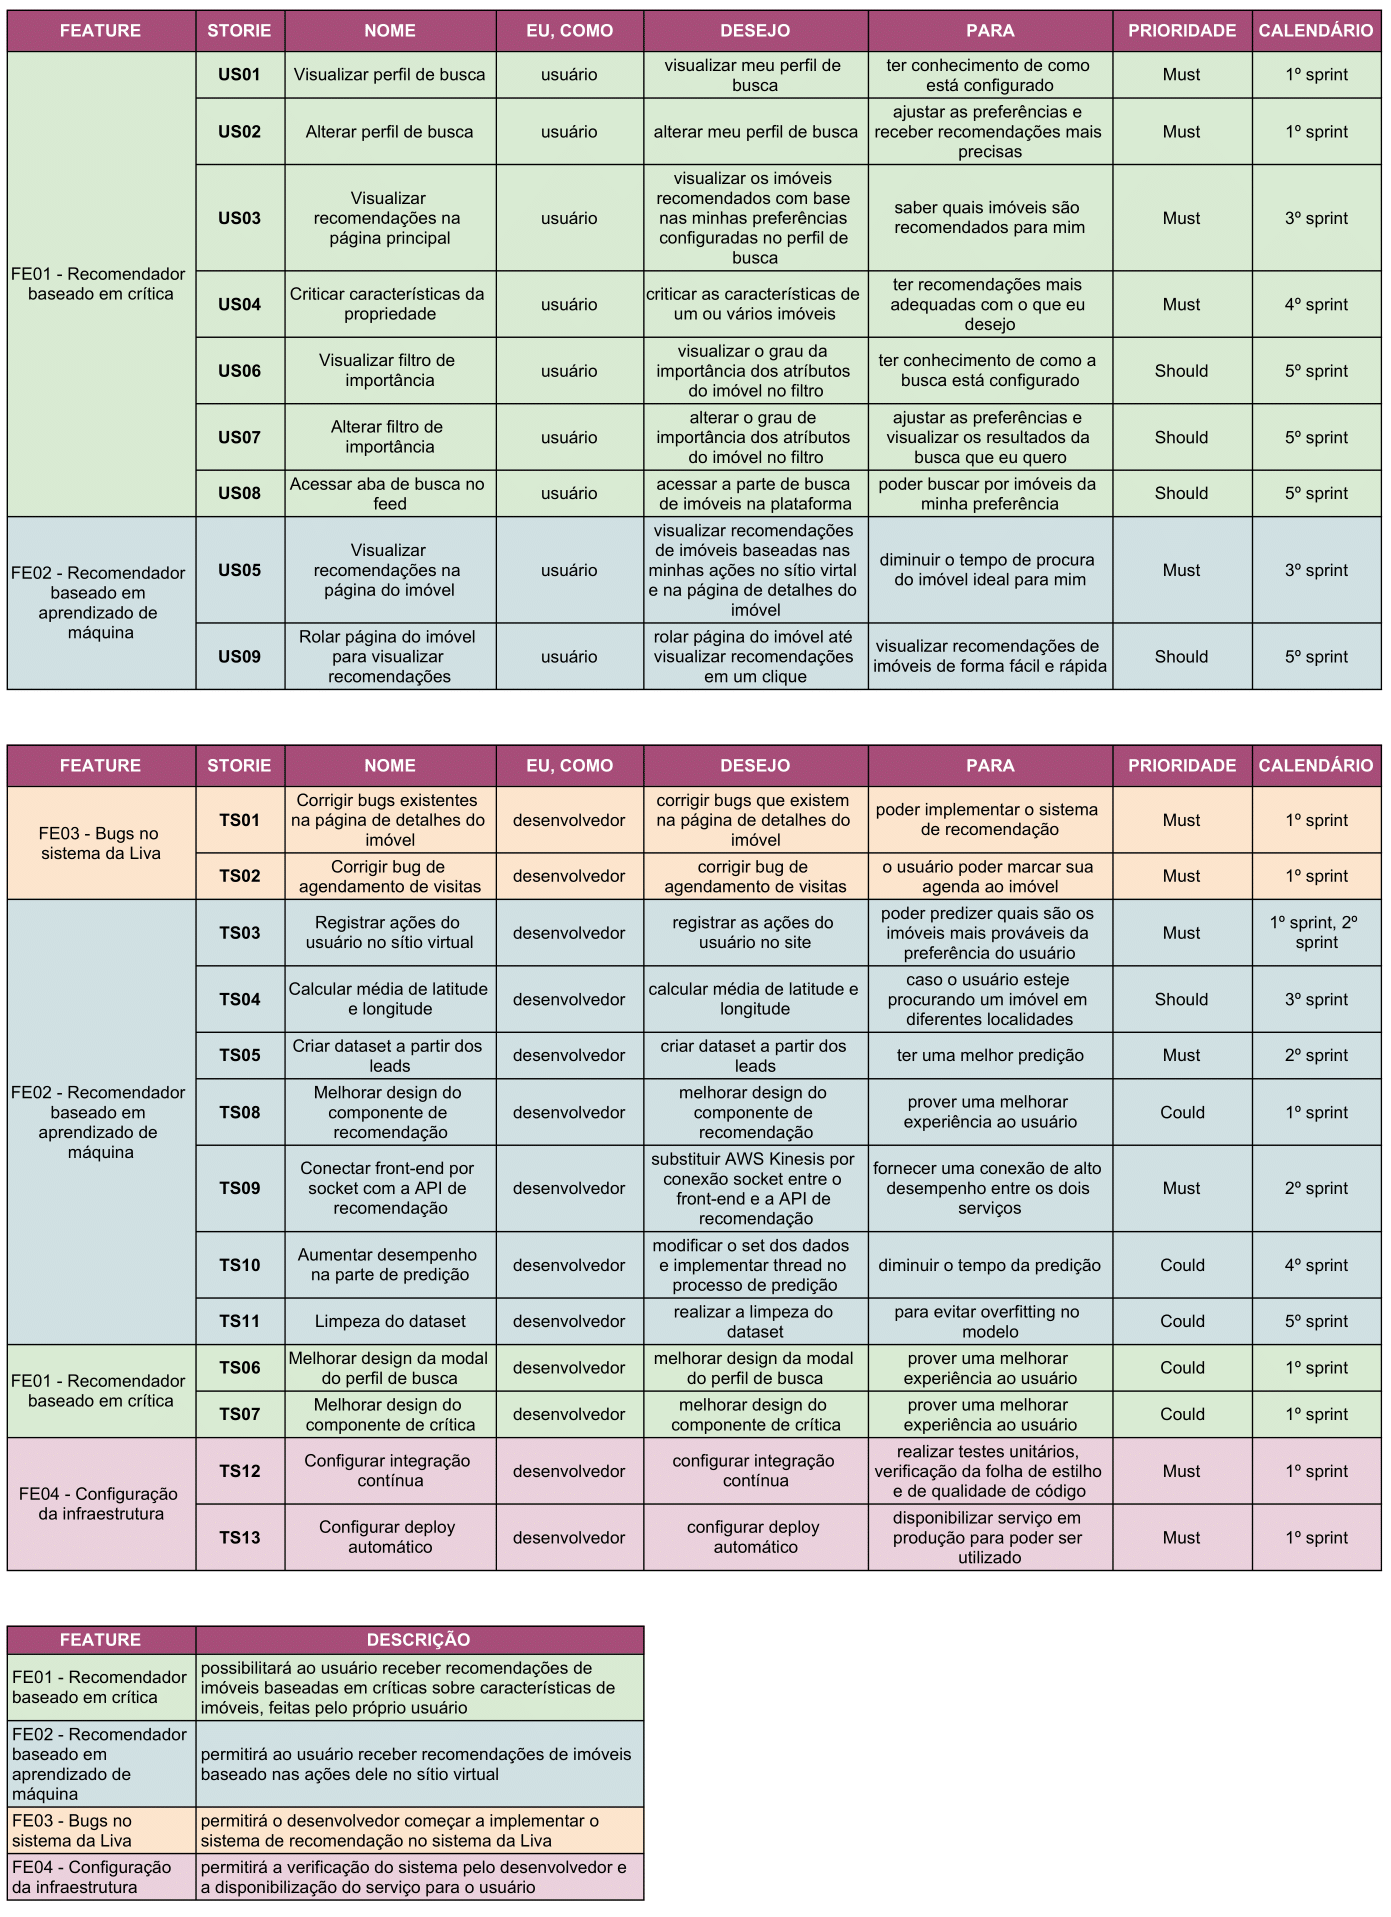
\includegraphics[scale=0.315]{figuras/desenvolvimento/Backlog.png}
    \caption[Backlog do produto atualizado]{Backlog do produto atualizado.}
    \label{fig:apendice_backlog}
\end{figure}

\chapter{Simulação da Proposta}
\label{apendiceA}

\section{Introdução}

Com o objetivo de validar a aplicabilidade da proposta, foi desenvolvido um protótipo , com partes disponíveis no Apêndice A deste trabalho. Para o desenvolvimento desse protótipo, como a solução se baseia em duas abordagens diferentes (módulo de critica e módulo de aprendizado de máquina), foi decidido fazer a implementação das duas de forma reduzida e minimalista. De forma geral, para o recomendador baseado em critica foi disponibilizado para o usuário uma pergunta que servirá para criticar apenas uma característica do imóvel, como apresentado nas Figuras \ref{fig:prototipo_simulacao_critica1}, \ref{fig:prototipo_simulacao_critica2} e \ref{fig:prototipo_simulacao_critica3}.

\begin{figure}[H]
    \centering
    
\includegraphics[scale=0.9]{figuras/consideracoes_finais/prototipo_simulacao_critica1.jpg}
    \caption[Protótipo da simulação da crítica parte 1]{Protótipo da simulação da crítica parte 1.}
    \label{fig:prototipo_simulacao_critica1}
\end{figure}

\begin{figure}[H]
    \centering
    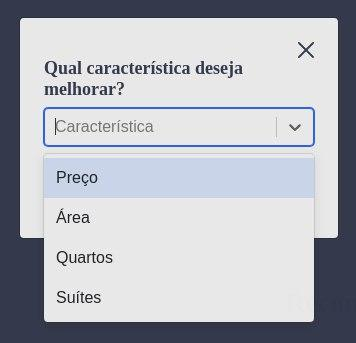
\includegraphics[scale=0.7]{figuras/consideracoes_finais/prototipo_simulacao_critica2.jpg}
    \caption[Protótipo da simulação da crítica parte 2]{Protótipo da simulação da crítica parte 2.}
    \label{fig:prototipo_simulacao_critica2}
\end{figure}

\begin{figure}[H]
    \centering
    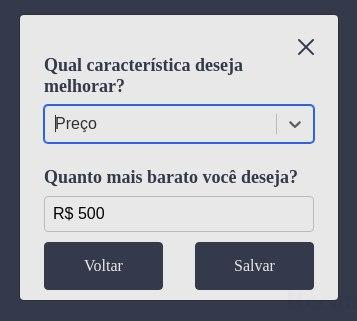
\includegraphics[scale=0.7]{figuras/consideracoes_finais/prototipo_simulacao_critica3.jpg}
    \caption[Protótipo da simulação da crítica parte 3]{Protótipo da simulação da crítica parte 3.}
    \label{fig:prototipo_simulacao_critica3}
\end{figure}

Dessa forma o usuário selecionará uma das características e atribuirá o valor de sua preferência. Em seguida, o perfil de busca do usuário será apropriado com base na crítica dessa característica em si, e assim serão geradas novas recomendações em seu \textit{feed}.

No recomendador de aprendizado de máquina foi decidido a construção de uma filtragem colaborativa baseado em modelo, utilizando-se da técnica de fatoração matricial, com o algoritmo de aprendizado de máquina Fatoração matricial não negativa (NMF) disponibilizado pela biblioteca scikit-learn. Para simular a integração do sistema de recomendação como um serviço, foi construída uma API própria para o protótipo. Seu \textit{deploy} foi feito por meio do serviço ECS do AWS, e tem um banco de dados próprio.Os dados de entrada do modelo foram retirados do banco de dados da Liva. Esses dados são referentes as ações de "Favoritar" e "Descartar" um imóvel feitas pelos usuários e foram copiados para o banco de dados da API.

Os dados dos usuários serão atualizados assim como modelo será treinado diariamente. A transformação da matriz que terá todos os usuário e todos os imóveis "avaliados", disponibilizará uma pontuação para cada propriedade. Dessa forma será possível recomendar para todos os usuários as cinco melhores propriedades geradas pelo algorítimo. Essas recomendações são apresentadas na página de detalhes do imóvel, assim como na solução proposta, e por meio de um componente carrossel do ReactJS chamado "\textit{swiper}" como na Figura \ref{fig:prototipo_simulacao_rs}.

\begin{figure}[H]
    \centering
    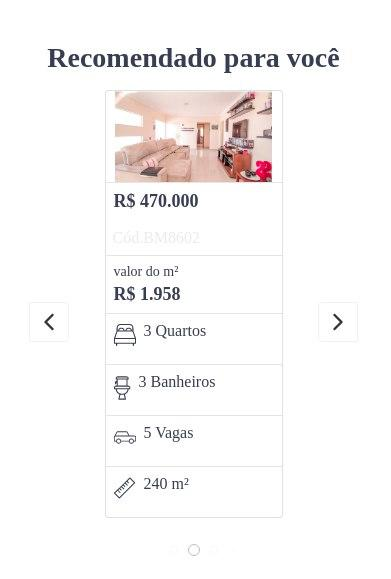
\includegraphics[scale=0.6]{figuras/consideracoes_finais/prototipo_simulacao_rs.jpg}
    \caption[Protótipo do sistema de recomendação]{Protótipo do sistema de recomendação.}
    \label{fig:prototipo_simulacao_rs}
\end{figure}

Foram obtidos dados por meio da ferramenta Mixpanel em integração com o \textit{front-end} da Liva. Esses dados referem-se a consultas realizadas pelo usuário dado um período de tempo. São registradas a frequência de acesso ao \textit{feed}, visualização na pagina de detalhes, edição do perfil de busca, avaliação (favoritar ou descartar) de um imóvel, solicitação de mais imóveis a serem recomendados no \textit{feed}, alteração de ação de favoritar ou descartar imóvel dentre outros. Além disso, foram separados todas as recomendações feitas para os usuários do banco de dados da Liva.

O protótipo ficou em produção do dia 26 ao dia 27 de novembro. Assim o resultado obtido foi comparado com os dois dias da semana anterior (19 e 20 de novembro). Abaixo (Tabela \ref{tab:my-table}) se encontra a representação dos dados obtidos.

\begin{table}[H]
\centering
\caption[Quantidade de recomendações, imóveis favoritados e descartados]{Quantidade de recomendações, imóveis favoritados e descartados.}
\begin{tabular}{lcc}
\hline
\textbf{Data do inicio - Data do fim} & 19/11/19 - 20/11/19 & 26/11/19 - 27/11/19 \\ \hline
\textbf{Quantidade de recomendações} & 715 & 537 \\ \hline
\textbf{Quantidade de imóveis favoritados} & 0 & 6 \\ \hline
\textbf{Quantidade de imóveis descartados} & 19 & 7 \\ \hline
\end{tabular}
\label{tab:my-table}
\end{table}

% 421 - recomendações
% 6 - likes
% 3 - dislikes
% 1.42

% 1055 - recomendações
% 10 - likes
% 12 - dislikes
% 0.94

\subsection{Analise dos resultados}

Com os dados obtidos foi possível analisar a aprovação das recomendações, medindo o grau de imóveis favoritados, dividindo o numero de imóveis recomendados favoritados pelo número total de recomendações multiplicado por 100, além do grau de imoveis descartados com o número de imóveis descartados, como mostrado na tabela \ref{tab:my-table2}.

\begin{table}[H]
\centering
\caption[Grau de imóveis favoritados e descartados]{Grau de imóveis favoritados e descartados.}
\begin{tabular}{lcc}
\hline
\textbf{Data do inicio - Data do fim} & 19 /11/19 - 20/11/19 & 26/11/19 - 27/11/19 \\ \hline
\textbf{Grau de imóveis favoritados} & 0.0 & 1.11 \\ \hline
\textbf{Grau de imóveis descartados} & 2.65 & 1.30 \\ \hline
\end{tabular}
\label{tab:my-table2}
\end{table}

Apesar do período pequeno da simulação, em virtude do encerramento do prazo para a finalização da primeira etapa (TCC1) e disponibilização para os avaliadores do trabalho, foi possível perceber uma melhora no grau de imoveis favoritados durante este breve período, com a aplicação e comparação dos dois recomendadores com abordagens diferentes, além de apresentar uma menor taxa de descartes.

\end{apendicesenv}